%----------------------------------------------------------------------------------------
%   PACKAGES AND OTHER DOCUMENT CONFIGURATIONS
%----------------------------------------------------------------------------------------
\documentclass[a5paper,pagesize,10pt,bibtotoc,DIV=10,twoside]{scrbook}

% twoside, openright
\KOMAoptions{DIV=last}

\usepackage[utf8]{inputenc}
\usepackage[T1]{fontenc}

\usepackage[pdftex]{graphicx}
\usepackage{amsmath}
\usepackage{amssymb}
\usepackage{tipa}
\usepackage{textcomp}
\PassOptionsToPackage{hyphens}{url}\usepackage{hyperref}
\usepackage{microtype}
\usepackage{libertine}

\usepackage{tocloft}
\usepackage{anyfontsize}
\usepackage{t1enc}

\usepackage[pagestyles]{titlesec}
\usepackage{fancyhdr}
\usepackage[none]{hyphenat}
\usepackage{float}
\usepackage{wrapfig}
\usepackage{csquotes}

\usepackage{relsize}
\renewcommand*{\UrlFont}{\ttfamily\smaller\relax}

\usepackage{multirow}

\titleclass{\subsubsubsection}{straight}[\subsection]

\usepackage{eso-pic}
\newcommand\BackgroundPic{%
\put(0,0){%
\parbox[b][\paperheight]{\paperwidth}{%
\vfill
\centering

\includegraphics[width=\paperwidth,height=\paperheight,keepaspectratio]{images/BookCover.png}
\vfill
}}}

\let\cleardoublepage\clearpage
\titlespacing*{\chapter}{0pt}{-60pt}{20pt}
\titlespacing*{\section}{10pt}{10pt}{5pt}
\titlespacing*{\subsection}{5pt}{5pt}{5pt}
\titleformat*{\section}{\large\bfseries}

\titleformat{\chapter}[display]
  {\normalfont\bfseries}{}{0pt}{\large}
\pagestyle{fancy}

\fancyhf{}
\fancyhead[RE]{\leftmark}
\fancyhead[LO]{\rightmark}
\fancyhead[LE,RO]{\thepage}
\renewcommand\headrulewidth{0pt}
\renewcommand\chaptermark[1]{\markboth{#1}{}} 
\renewcommand\sectionmark[1]{\markright{\thesection.\ #1}}


\renewcommand\cftchapfont{\large\bfseries}
\renewcommand\cftsecfont{\normalsize}
\renewcommand\cftsubsecfont{\normalsize}

\renewcommand\cftchappagefont{\large\bfseries}
\renewcommand\cftsecpagefont{\normalsize}
\renewcommand\cftsubsecpagefont{\normalsize}

\renewcommand\thesubsection{}

\definecolor{must}{RGB}{250, 0, 38}
\definecolor{should}{RGB}{228, 86, 60}
\definecolor{could}{RGB}{255, 140, 0}
\definecolor{safe}{RGB}{124, 10, 2}

\usepackage[acronym]{glossaries}
\makeglossaries

\newglossaryentry{SAFE}{
    name=SAFE,
    description={Sensitive, Access-Controlled, Foolproof, Enforced}
}


\begin{document}

%----------------------------------------------------------------------------------------
%   TITLE PAGE
%----------------------------------------------------------------------------------------

\begingroup
\thispagestyle{empty}
\AddToShipoutPicture*{\BackgroundPic}
\endgroup

%----------------------------------------------------------------------------------------
%   COPYRIGHT PAGE
%----------------------------------------------------------------------------------------

\newpage
~\vfill
\thispagestyle{empty}

\newpage

\begin{center}


\vspace{100mm}
Brought to you by:\par
\large \textsc{??? \\}
\vspace{10mm}
\normalsize{?}\par

\end{center}
\vspace{110mm}



\small \noindent \textsc{London, United Kingdom}\\
\tiny \noindent \textit{First release, September 2017}\\

\vspace{5mm}
\tiny \noindent \textsc{\url{https://wiki.iggroup.local/display/APPSEC/Application+Security+Home}}

%----------------------------------------------------------------------------------------
%   TABLE OF CONTENTS
%----------------------------------------------------------------------------------------
\newpage
\tableofcontents
\newpage

\normalsize

%----------------------------------------------------------------------------------------
%   INTRODUCTION
%----------------------------------------------------------------------------------------
\chapter{Introduction}

\section{About This Book}
Application security is increasing becoming a critical focus for software developers. This booklet distils the key elements of application security principles, defences and practices. \\

\section{Foolish Assumptions}
We assume you are a software developer with some interest in making sure your applications are secure. \\

\section{OWASP}

Everything you read here is derived directly or indirectly from the Open Web Application Security Project - \url{www.owasp.org}, a  worldwide not-for-profit charitable organisation focused on improving software security.\\

%----------------------------------------------------------------------------------------
%   REASON
%----------------------------------------------------------------------------------------
\chapter{The Reason}

\section{Why do we need application security?}

We need application security because we are building applications, and the threat of security breaches (whether deliberate or accidental) is real. The diagram\cite{breaches} below shows a snapshot of the world's biggest data breaches in recent years. You don't want your application to be the reason your company ends up on this list. \\

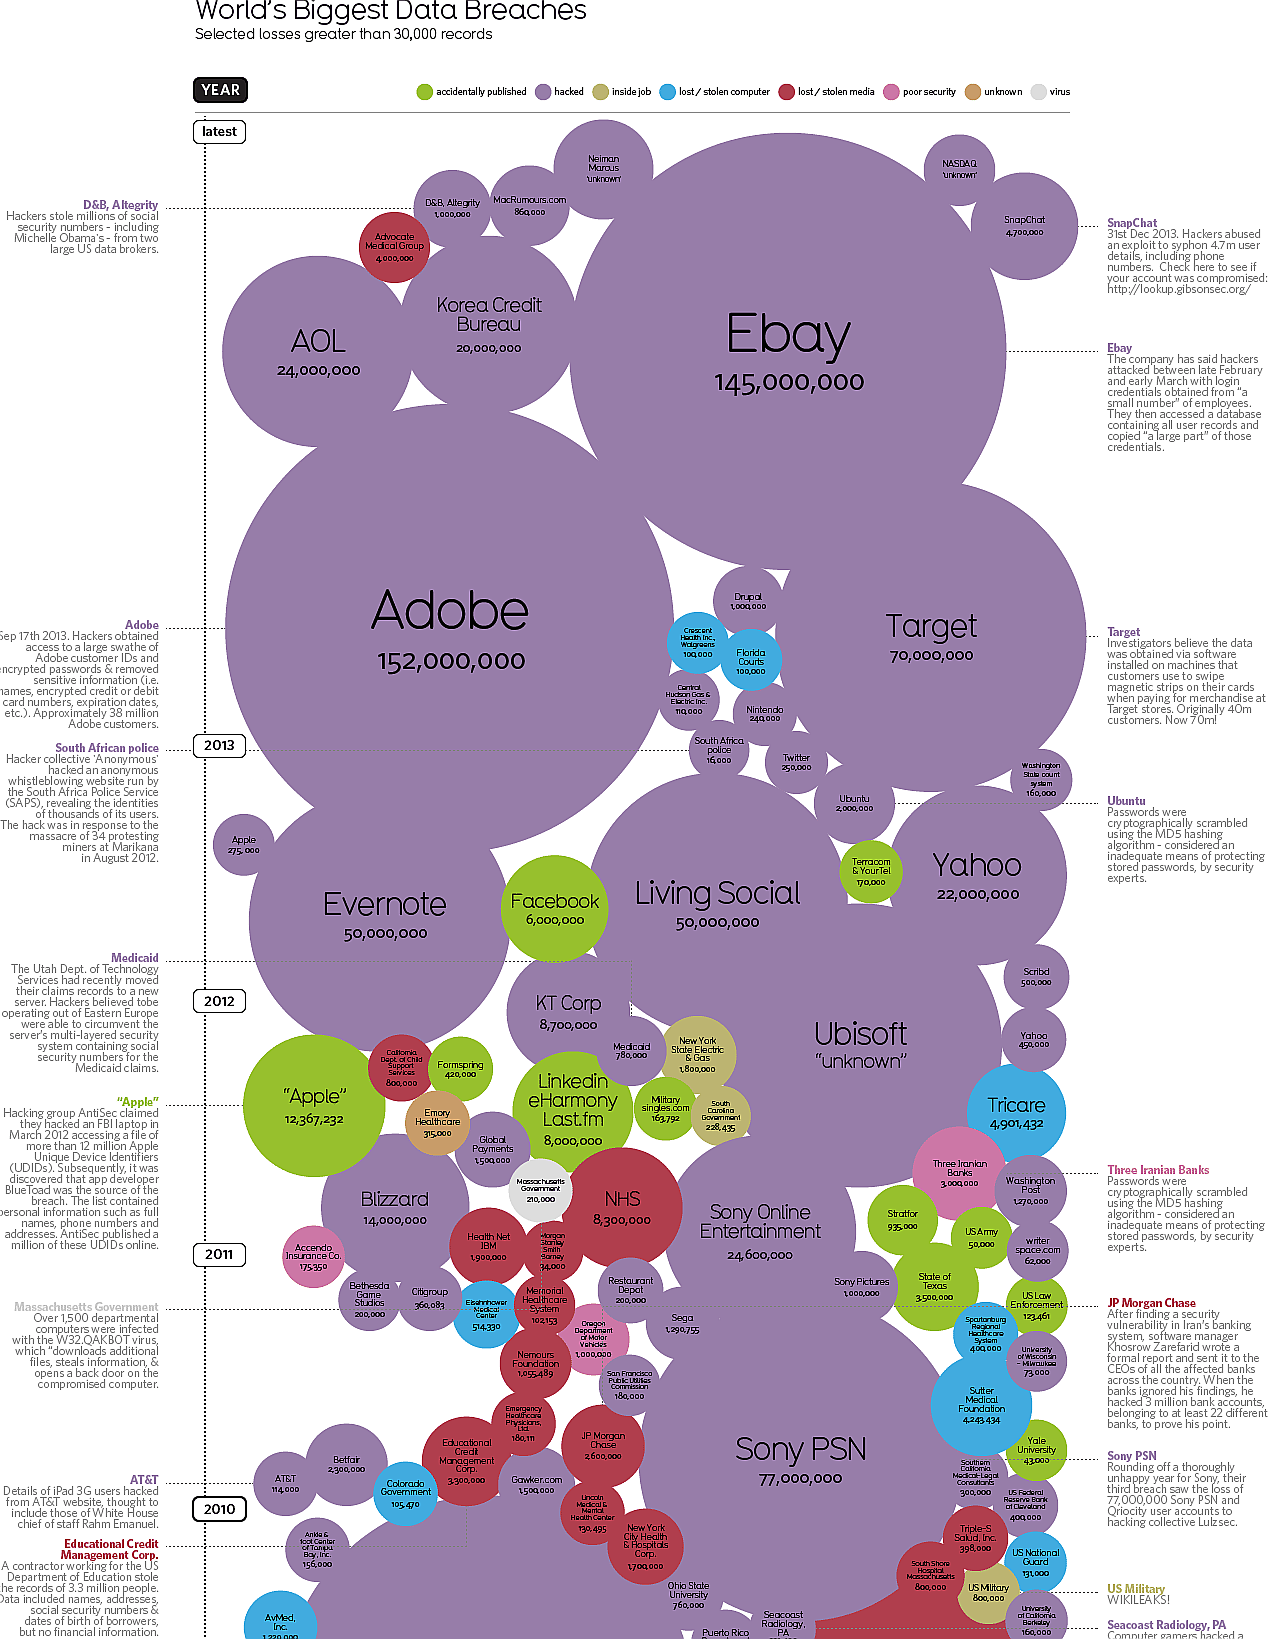
\includegraphics[scale=0.277]{images/breaches-edited}


Apart from maintaining the reliability, integrity and availability of our systems, any company has a reputation to uphold, customers and confidential data to preserve, and regulatory bodies to keep happy. 

\section{What are ydour secrets?}

Some typical examples of assets that applications need to protect include: client usernames, passwords and personally identifiable information (PII) such as names, addresses, credit card details; system passwords and certificates; session tokens; market information (prices).

\section{Who are the threat agents?}

Anyone is potentially a threat. Here are some typical threat agents:

\begin{figure}[H]
\centering
\includegraphics[scale=0.4]{images/ThreatAgents}
\end{figure}

These include not just hackers and customers, but also employees, who may be careless or targeted by criminals. The availability of sensitive assets to employees, contractors or partners opens up a whole new world of risks regarding access and use of available data. \\ 

The following chart from Forrester shows the most common breaches from surveys sent out to US companies, with almost \textbf{40\%} being \textbf{internal incidents}. We need to protect our systems against breaches from all sides.\\

\begin{figure}[htbp]
\hspace*{-1.5cm} 
\includegraphics[scale=0.26]{images/Forrester}
\end{figure}


%----------------------------------------------------------------------------------------
%   ATTACK
%----------------------------------------------------------------------------------------
\chapter{The Attack}
Thinking like a hacker is fundamental to good application security.

%----------------------------------------------------------------------------------------
%   STRIDE
%----------------------------------------------------------------------------------------
\section{STRIDE}

\textit{Microsoft} introduced the \textbf{STRIDE} threat modeling process in 1999, where systems are analysed with respect to the threats of: \\

\begin{itemize}
\item \textbf{S}poofing
\item \textbf{T}ampering
\item \textbf{R}epudiation 
\item \textbf{I}nformation disclosure 
\item \textbf{D}enial of service 
\item \textbf{E}levation of privilege.
\end{itemize}

\subsection{Spoofing}

Spoofing is when a malicious entity impersonates another device/user on the network in order to bypass access controls, steal data or start attacks against other hosts on the network.\\

There are two types of spoofing attacks:

\begin{itemize}
\item Identity spoofing: means you are pretending to be someone you are not. Examples include: theft or brute force hacking of user credentials, or session hijacking.
\item Origin spoofing: IP, ARP and DNS spoofing attacks refer to using false source addresses to transmit data or modifying DNS servers in order to reroute a specific domain name to a different address. 
\end{itemize}

\subsection{Tampering}

Tampering means taking a valid request and changing it in some way that benefits the attacker.  Examples of tampering include: injecting code into text fields to achieve malicious intent, or unauthorized changes to persistent data from a database. 

\subsection{Repudiation}

Repudiation means denying a truth, such as something that has happened.  An example of this might be a customer claiming that they transferred more money than they actually did.\\
\textbf{Nonrepudiation} is the ability of a system to counter repudiation threats.

\subsection{Information Disclosure}

Information disclosure means exposing sensitive data to users or systems that are not supposed to have access to it. Examples include reading data in transit between two computers, in log files, or accessing data directly in the database. 

\subsection{Denial of Service}

This type of attack targets valid users that are denied access to a given system. An example is flooding a database server with TCP/IP packets and rendering the service temporarily unavailable or unusable, or locking user accounts.

\subsection{Elevation of Privilege}

Also called privilege escalation, this is a type of threat that allows unprivileged users to get access and sufficient permissions needed to compromise or destroy entire systems. 


%----------------------------------------------------------------------------------------
%   OWASP TOP 10
%----------------------------------------------------------------------------------------
\section{OWASP Top 10}

\textbf{TO DO: Rebase on OWASP Top 10 \textit{2017}} 

\textsc{\normalsize\textbf{The Ten Most Critical Web Application Security Risks}}\\

OWASP Top 10 (\textbf{2017}) is an awareness document for web application security. It represents a broad consensus on the most critical application security risks. \\

If your app is a mobile app then you should use the OWASP Mobile Top 10 (\url{https://wiki.iggroup.local/display/APPSEC/OWASP+Mobile+Top+10}) instead. (to expand)

%----------------------------------------------------------------------------------------
%   A1
%----------------------------------------------------------------------------------------
\subsection{\textit{A1} \normalsize{Injection}}

\fbox{\begin{minipage}{1.0\textwidth}
Injection flaws, such as \textbf{JavaScript}, \textbf{SQL}, \textbf{OS}, and \textbf{LDAP} injection occur when untrusted data is sent to an interpreter as part of a command or query. The attacker’s hostile data can trick the interpreter into executing unintended commands or accessing data without proper authorisation.
\end{minipage}}

\vspace{2mm}
\textbf{Attack scenarios: JavaScript injection attacks - \textbf{TO DO:} change examples}


\begin{itemize}

\item Possible if the client browser has the ability to interpret scripts embedded within HTML content enabled by default. So if an attacker embeds script tags such \big\langle\verb|SCRIPT|\big\rangle, \big\langle\verb|OBJECT|\big\rangle, \big\langle\verb|APPLET|\big\rangle, or \big\langle\verb|EMBED|\big\rangle into a web site, the web browser's JavaScript engine will execute it.

\item Insert JavaScript code in the page URL, modifying the behaviour of the page:

\end{itemize}


%----------------------------------------------------------------------------------------
%   A2
%----------------------------------------------------------------------------------------
\subsection{\textit{A2}  \normalsize{Broken Authentication}}

\fbox{\begin{minipage}{1.0\textwidth}
Application functions related to authentication and session management are often not implemented correctly, allowing attackers to compromise passwords, keys, or session tokens, or to exploit other implementation flaws to assume other users’ identities.
\end{minipage}}

\newpage
\textbf{Attack scenario  \textbf{TO DO:} change examples}\\
\begin{itemize}
\item Session (SSO) tokens expire every few hours, rather than seconds. Therefore, they are at risk from leakage, for example, in URLs and  logs.
\end{itemize}


%----------------------------------------------------------------------------------------
%   A3
%----------------------------------------------------------------------------------------
\subsection{\textit{A3}  \normalsize{Sensitive Data Exposure}}

\fbox{\begin{minipage}{1.0\textwidth}

\end{minipage}}

\vspace{15mm}
\textbf{Attack scenarios  \textbf{TO DO:} change examples}\\

\begin{itemize}
\item \textbf{Reflected XSS: }\cite{reflected-xss}
\begin{figure}[H]
\includegraphics[scale=0.35]{images/reflected-xss}
\end{figure}
\item \textbf{Stored XSS: }\cite{stored-xss}
\begin{figure}[H]
\includegraphics[scale=0.35]{images/xss}
\end{figure}
\end{itemize}


%----------------------------------------------------------------------------------------
%   A4
%----------------------------------------------------------------------------------------
\subsection{\textit{A4}  \normalsize{XML External Entities (XXE)}}

\fbox{\begin{minipage}{1.0\textwidth}
Many older or poorly configured XML processors evaluate external entity references within XML
documents. External entities can be used to disclose internal files using the file URI handler,
internal file shares, internal port scanning, remote code execution, and denial of service attacks. (TO DO: rewrite)
 \end{minipage}}
 
\textbf{Attack scenario \textbf{TO DO:} change examples}
\vspace{-5mm}
\begin{itemize}
\item An altered call to obtain another user's statement: \cite{insecure}\\
\includegraphics[scale=0.4]{images/a4}
\end{itemize}


%----------------------------------------------------------------------------------------
%   A5
%----------------------------------------------------------------------------------------
\subsection{\textit{A5}  \normalsize{Broken Access Control}}

\fbox{\begin{minipage}{1.0\textwidth}

\end{minipage}}

\includegraphics[scale=0.4]{images/a5-illustr} \cite{a5}

\newpage
\textbf{Attack scenarios \textbf{TO DO:} change examples}

\begin{itemize}
\item Poorly configured application properties across various environments
\item Default settings for applications, frameworks and servers
\item Returning full stack traces exposing application flaws
\item Storing build artifacts in insecure network locations
\item Directory listing not disabled on the server:\\

\includegraphics[scale=0.4]{images/a5-list}
\end{itemize}


%----------------------------------------------------------------------------------------
%   A6
%----------------------------------------------------------------------------------------
\subsection{\textit{A6}  \normalsize{Security Misconfiguration}}

\fbox{\begin{minipage}{1.0\textwidth}
Good security requires having a secure configuration defined and deployed for the application, frameworks, application server, web server, database server, and platform. Secure settings should be defined, implemented, and maintained, as defaults are often insecure. Additionally, software should be kept up to date. 
Many web applications do not properly protect sensitive data, such as credit cards, tax IDs, and authentication credentials. Attackers may steal or modify such weakly protected data to conduct credit card fraud, identity theft, or other crimes. Sensitive data deserves extra protection such as encryption at rest or in transit, as well as special precautions when exchanged with the browser. 
\end{minipage}}

\vspace{7mm}
\includegraphics[scale=0.3]{images/a6} \cite{a6}

\vspace{2mm}
\textbf{Attack scenarios \textbf{TO DO:} change examples}

\begin{itemize}
\item A web app does not use SSL for all authenticated pages, allowing attackers to monitor network traffic, steal session cookies and perform reply attacks to steal users' sessions
\item Session tokens on GET requests are logged
\end{itemize}


%----------------------------------------------------------------------------------------
%   A7
%----------------------------------------------------------------------------------------
\subsection{\textit{A7}  \normalsize{Cross-Site Scripting (XSS)}}

\fbox{\begin{minipage}{1.0\textwidth}
XSS flaws occur whenever an application takes untrusted data and sends it to a web browser without proper validation or escaping. XSS allows attackers to execute scripts in the victim’s browser which can hijack user sessions, deface web sites, or redirect the user to malicious sites.
Web applications often verify function level access rights before making that functionality visible in the UI. However, applications need to perform the same access control checks on the backend server when each function is accessed. If requests are not verified, attackers will be able to forge requests in order to access functionality without proper authorisation.
\end{minipage}}

\vspace{2mm}
\textbf{Attack scenario \textbf{TO DO:} change examples}

\begin{itemize}
\item An attacker can force-browse to various target URLs in order to determine which pages are visible (to both authenticated/unauthenticated users) \\

\begin{figure}[htbp]
\hspace*{-0.5cm} 
\includegraphics[scale=0.52]{images/a7}
\end{figure}

\end{itemize}


%----------------------------------------------------------------------------------------
%   A8
%----------------------------------------------------------------------------------------
\subsection{\textit{A8}  \normalsize{Insecure Deserialization}}

\fbox{\begin{minipage}{1.0\textwidth}
A CSRF attack forces a logged-on victim's browser to send a forged HTTP request, including the victim's session cookie and any other automatically included authentication information, to a vulnerable web application. This allows the attacker to force the victim's browser to generate requests the vulnerable application thinks are legitimate requests from the victim.
\end{minipage}}

\includegraphics[scale=0.6]{images/csrf}

CSRF takes advantage of the fact that most web applications allow attackers to predict all the details of a particular action. Browsers send credentials like session cookies automatically. Therefore, attackers can create malicious web pages which generate forged requests that are indistinguishable from legitimate ones.\\

\textbf{Attack scenarios \textbf{TO DO:} change examples}

\begin{itemize}
\item An attacker constructs a request to transfer funds from the victim's account to the attacker's account and embeds it in an image request or iframe stored on malicious sites:\\
\small{\big\langle\verb|img src="http://example.com/app/transferFunds?|}\\
\small{\verb|amount=1500\&destination|}\\
\small{\verb|Account=attackersAcct\#" width="0" height="0"|\big\rangle}
\item When the victim visits one of the attacker's sites and is still authenticated on example.com, the request above will send back session and authentication information as well as authorise the embedded request.
\end{itemize}


%----------------------------------------------------------------------------------------
%   A9
%----------------------------------------------------------------------------------------
\subsection{\textit{A9}  \normalsize{Using Components with Known Vulnerabilities}}

\fbox{\begin{minipage}{1.0\textwidth}
Components, such as libraries, frameworks, and other software modules, almost always run with full privileges. If a vulnerable component is exploited, such an attack can facilitate serious data loss or server takeover. Applications using components with known vulnerabilities may undermine application defenses and enable a range of possible attacks and impacts.
\end{minipage}}

\vspace{2mm}
\textbf{Attack scenario \textbf{TO DO:} change examples}

\begin{displayquote}
\textbf{"A system is only as strong as its weakest link."}\\

\end{displayquote}

%----------------------------------------------------------------------------------------
%   A10
%----------------------------------------------------------------------------------------
\subsection{\textit{A10}  \normalsize{Insufficient Logging\&Monitoring}}

\fbox{\begin{minipage}{1.0\textwidth}
Web applications frequently redirect and forward users to other pages and websites, and use untrusted data to determine the destination pages. Without proper validation, attackers can redirect victims to phishing or malware sites, or use forwards to access unauthorized pages.
\end{minipage}}

\vspace{2mm}
\textbf{Attack scenario \textbf{TO DO:}change examples}
\begin{itemize}
\item Redirect URL:\\
\small{\verb|http://www.example.com/redirect.jsp?url=evil.com|}
\end{itemize}



%----------------------------------------------------------------------------------------
%   DEFENCE
%----------------------------------------------------------------------------------------
\chapter{The Defence}

%----------------------------------------------------------------------------------------
%   GOALS
%----------------------------------------------------------------------------------------
\section{Security Goals}

Information Security relies on three core pillars, also known as the CIA triad: 

\begin{itemize}
\item \textbf{Confidentiality}: only allow access to data for which the user is permitted
\item \textbf{Integrity}: ensure data is not tampered or altered by unauthorized users
\item \textbf{Availability}: ensure systems and data are available to authorized users when they need it
\end{itemize}

\begin{wrapfigure}{r}{0.45\textwidth}
\includegraphics[width=0.4\textwidth]{images/CIA}
\end{wrapfigure}

The following security principles and measures are based on these three pillars and outline proven examples of theoretical security principles used in the software development lifecycle.\\

%----------------------------------------------------------------------------------------
%   PRINCIPLES
%----------------------------------------------------------------------------------------
\section{Security Principles}

\subsection{Apply defence in depth}
The principle of defence-in-depth is that layered security mechanisms increase security of the system as a whole. If an attack causes one security mechanism to fail, other mechanisms may still provide the necessary security to protect the system.

\subsection{Use a positive security model}
A \textbf{positive} security model (also known as \textit{whitelist}) is one that defines what is allowed, and rejects everything else. This should be contrasted with a "negative" (or \textit{blacklist}) security model, which defines what is disallowed, while implicitly allowing everything else. The benefit of using a positive model is that new attacks, not anticipated by the developer, will be prevented. 

\subsection{Fail securely}
Handling errors securely is a key aspect of secure coding. In general, you should design your security mechanism so that a failure will follow the same execution path as disallowing the operation. Also, avoid leaking system information in error messages presented back to the caller.

\subsection{Run with least privilege}
The principle of least privilege recommends that accounts have the least amount of privilege required to perform their business processes. 

\subsection{Avoid security by obscurity}
Obscurity offers no hurdle to a determined hacker. Avoid it.

\subsection{Keep security simple}
Attack surface area and simplicity go hand in hand. The more difficult it is to reason about your system, the less likely it is to be secure.

\subsection{Detect intrusions}
Detecting intrusions requires three elements:
\begin{itemize}
\item the capability to log security-relevant events
\item procedures to ensure the logs are monitored regularly
\item procedures to properly respond to an intrusion once detected
\end{itemize}

\subsection{Don't trust infrastructure}
Don't rely only on infrastructure to secure your system.

\subsection{Don't trust services}
Trust increases coupling and vulnerability. Don't blindly trust any data your receive.

\subsection{Establish secure defaults}
Users may opt to reduce security, but by default, systems should be secure.

\subsection{Fix security issues correctly}
Once a security issue has been identified, it is important to develop a test for it, and to understand the root cause of the issue.



%----------------------------------------------------------------------------------------
%   MEASURES
%----------------------------------------------------------------------------------------
\section{Security Measures - \textbf{TO DO:} rewrite/redo picture}


Note that security is applicable to every remotely accessible endpoint, regardless of where it is hosted. \\

\subsection{Zoning}
Applications/services must be hosted in the appropriate DMZ (Frontend, Middleware, or Backend).

\subsection{Authentication}
\begin{itemize}
\item Always identify the caller
\item Require \textit{explicit} access tokens, preferably in the header.
\item Avoid tokens in URLs, as they will be logged by web servers. Obfuscate if you have no choice, or use short-lived tokens.
\item Avoid relying on cookies for authentication, as they allow CSRF attacks.
\end{itemize}

\subsection{Authorisation}
\begin{itemize}
\item Always check that the caller has appropriate rights, both to the function and the data
\item Remember not all access tokens are created equal. Distinguish between client and service access accounts. Always prefer client credentials as they enable more appropriate authorisation of requests
\end{itemize}

\subsection{Auditing}

Log requests, remembering to exclude sensitive data

\subsection{Confidentiality}
Preventing disclosure of information to unauthorised users or systems, e.g. by:
\begin{itemize}
\item Encrypting sensitive communications
\item Encrypted storage of sensitive data
\item Secured/audited access to storage areas and servers
\item Not logging sensitive data
\item Not storing secrets in source code
\end{itemize}

\subsection{Cryptography}
Don't write your own security libraries.

\subsection{Integrity}
Ensure critical information cannot be modified without detection, e.g. by using digital signatures.

\subsection{Non-repudiation}
Ensure that someone cannot dispute the fact they sent a specific message, e.g. by digitally signing information or auditing requests.

\subsection{Secure Movement}
Use encrypted channels, TLS for point to point. Multiple step messaging will require additional measures, such as:

\begin{itemize}
\item payload encryption (to protect message contents, or as a means of end to end authentication using certficates
\item payload dating and signing to avoid tampering or replay attacks
\end{itemize}

\subsection{Validation}
\begin{itemize}
\item Prevent script injection and buffer overflow type attacks
\item Never blindly trust the input. Perform server-side data validation (using strongly-typed fields, or failing that, strings with defined format, known-good character lists, or known-bad character lists). Don't forget to perform business rule validation.
\item This also applies to data sources like news feeds or content creation systems that are potentially untrustworthy
\end{itemize}

\subsection{Whitelisting}
Add further protection to highly sensitive endpoints by limiting source IP addresses or hostnames to a white list.

\subsection{Secure Storage}
\begin{itemize}
\item Do not store Highly Confidential customer data in widely accessibly areas (e.g. source code, unrestricted file system)
\item Debug logging of essential customer data is permissible only if required for support purposes.  Ensure that INFO level logging is on by default in production
\item Error logging of essential customer data is permissible in Production \textbf{only} if required for support purposes. Convenience is not a sufficient requirement.
\end{itemize}

\subsection{Appropriate Retention}
Ensure compliance with the Data Retention Policy, paying particular attention to the sections on customer account, dealing and payment information data.

\subsection{Secure Failure}
\begin{itemize}
\item Don't leak system information that could be useful to attackers
\item Catch internal errors, log them with a unique GUID, and return that to the caller
\end{itemize}


\newpage
%----------------------------------------------------------------------------------------
%   PRACTICES
%----------------------------------------------------------------------------------------
\section{Security Practices}

Addressing security in every stage of the Software Development Life Cycle is necessary in order to minimise risks and avoid vulnerabilities. The further along security issues are discovered, the bigger and costlier their impact.\\
\begin{figure}[H]
\hspace*{-1cm} 
\includegraphics[scale=0.53]{images/sdlc2} \cite{sdlc}
\end{figure}

With the rise in the intensity and the number of attack vectors, it has become necessary for organisations to include security as part of every phase of an SDLC:\\
\begin{figure}[H]
\includegraphics[scale=0.5]{images/ssdlc1}
\end{figure}



%----------------------------------------------------------------------------------------
%   POLICIES
%----------------------------------------------------------------------------------------
\subsection{\textbf{i.} Information Security Policies and Guidelines}



%----------------------------------------------------------------------------------------
%   SDLC
%----------------------------------------------------------------------------------------
\subsubsection{?? }

\begin{itemize}

\item \textit{Traceable change}
%: It is important that any change we introduce can be traced back to those who made and approved the change, along with the rationale for the change - which environment it is being released to, its impact, the project/request/incident/risk it is related to, its milestones and overall timeline.

\item \textit{Risk assessed security}
%: Creating and supporting software has inherent security risks that must be dealt with in an effective manner: all systems must be tested against relevant threats, projects must be assessed against security risks - cataloged, prioritised, dealt with as part of project delivery.

\item \textit{Automated quality assurance}
%: Automated quality gates enable us to introduce changes with confidence. Some examples of quality assessments include quality metrics for functional and non-functional requirements, in place monitoring with proactive resolution steps defined to prevent failures and automated security tests. 

\item \textit{Considered architecture}
%: We need to ensure we structure our software in the right way and use the right tools for the job. Every project is assessed from an architecture point of view for performance, scalability, resilience, availability, security and compliance with stated architectural goals, principles and patterns.

\item \textit{Sustainable delivery}
%: In order to make commitments to release software at predictable times we need to be sustainable in our approach: deployments and releases must be consistent, repeatable and scripted, rollback procedures must be tested. 

\item \textit{Fit for purpose solutions}
%: Software we create must be suitable for its intended purpose: code is reviewed, changes are signed off by QAs and when a piece of software is decommission, a retirement plan will be put in place.
\end{itemize}



%----------------------------------------------------------------------------------------
%   RISK ASSESSMENT
%----------------------------------------------------------------------------------------
\subsection{\textbf{ii.} Security Risk Assessment}

Key application security risks, as defined by OWASP. For each risk identified, it describes the actions being taken to mitigate the risk:
\begin{itemize}
\item Secure Coding Practices and Configuration

\item Internal Vulnerability Assessments and Third-Party Penetration Tests
\item Server Build Standard Vulnerability Assessments and Hardening
\end{itemize}


%----------------------------------------------------------------------------------------
%   THREAT MODELLING
%----------------------------------------------------------------------------------------
\subsection{\textbf{iii.} Threat Modelling}

Threat models \textbf{identify}, \textbf{quantify} and help \textbf{address} the vulnerabilities \textbf{early} in the development lifecycle.\\

Threat modelling helps you think like a hacker and produce and important form of documentation representing data flowing around your application, as follows:\\




%----------------------------------------------------------------------------------------
%   Decompose App
%----------------------------------------------------------------------------------------
\textsc{\textbf{Decompose App}}\\

Decomposing an app allows you to analyse its data flow. Ideally, you look at features rather than individual endpoints and the reason for this is it can help show how a small flaw in one part of your app can lead to a compromise in another. It should go without saying but, your decomposition should match reality. To make this process easier, you can use the following one-page threat model template:
\begin{figure}[H]
\includegraphics[scale=0.25]{images/threat1}\cite{threatModel}
\end{figure}

\textbf{Data flow diagram}\\

Start by creating a simple diagram showing the flow of data built from the following components:
\begin{figure}[H]
\includegraphics[scale=0.4]{images/DFD}
\end{figure}

In drawing the diagram, think about the \textbf{Assets} - what data you are trying to protect, \textbf{Threat Agents} - who the actors are that want to exploit your data, and \textbf{Trust Boundaries} involved - entry and exit points of your application, such as files, network, content management systems, deep-links etc.\\

%----------------------------------------------------------------------------------------
%   Determine Threats
%----------------------------------------------------------------------------------------
\textsc{\textbf{Determine threats}}\\

Once you have drawn up the data flow diagram, the next step is to come up with a list of threats by performing a risk assessment.\\

\textbf{How to determine Security Risks}\\

Use frameworks like \textbf{OWASP Top 10} and \textbf{STRIDE} to find vulnerabilities in your app.\\

%----------------------------------------------------------------------------------------
%   Rank Threats
%----------------------------------------------------------------------------------------
\textsc{\textbf{Rank threats}}\\

Use the \textbf{OWASP Risk Rating Methodology}, which breaks down likelihood and impact into much easier to answer questions. This is based on an Excel template available to make scoring easier. Reusable risk assessments are also available.

\begin{figure}[H]
\hspace*{-2.5cm}
\includegraphics[scale=0.29]{images/riskassessment}
\end{figure}

Factors for Estimating \textbf{Likelihood} - there are a number of factors that can help determine the likelihood. The first set of factors are related to the threat agent involved:

\begin{itemize}
\item Skill level
\item Motive
\item Opportunity
\item Size
\item Ease of discovery
\item Ease of exploit
\item Awareness
\item Intrusion Detection
\end{itemize}

Factors for Estimating \textbf{Impact} - again, each factor has a set of options:

\begin{itemize}
\item Loss of confidentiality
\item Loss of integrity
\item Loss of availability
\item Loss of accountability
\item Financial damage
\item Reputation damage
\item Non-compliance
\item Privacy violation
\end{itemize}

Determine the Severity of the Risk - based on the score acquired from previous steps:\\

$Risk = Likelihood * Impact$ \\
A quick way to rate a vulnerability is to rank likelihood and impact using Low, Medium or High categories: 
\begin{figure}[H]
\centering
\includegraphics[scale=0.7]{images/likelihood}
\end{figure}


%----------------------------------------------------------------------------------------
%   Mitigate Threats
%----------------------------------------------------------------------------------------
\textsc{\textbf{Mitigate threats}}\\

Even in scenarios where you are not fixing a vulnerability, it is also essential to ensure there is an audit trail of the decision.\\


%----------------------------------------------------------------------------------------
%   SECURITY NFRs
%----------------------------------------------------------------------------------------
\newpage
\subsection{\textbf{iv.} Security NFRs  \textbf{TO DO:} change image}

Security NFRs should include the following:


%----------------------------------------------------------------------------------------
%   SAFE CODE
%----------------------------------------------------------------------------------------
\subsection{\textbf{v.} SAFE Code  \textbf{TO DO:} change wording and picture}

\begin{figure}[H]
\includegraphics[scale=0.34]{images/safe}
\end{figure}

\newpage
\hspace*{-0.5cm}\textsc{\textbf{\textcolor{safe}{\textbf{Sensitive}} }} - Never log sensitive data \&  Never store secrets in source code 

\begin{itemize}
\item Remember that logs on servers are widely visible internally
\item Sensitive data primarily means session tokens and customer details that can be used to identify individuals
\item Beware of logging whole objects, or all headers, that may include sensitive data
\item Only use obfuscation as a short-term measure
\end{itemize}

\hspace*{-0.5cm}\textsc{\textbf{\textcolor{safe}{\textbf{Access-Controlled}} }} - Authenticate \& Authorise \& Audit

\begin{itemize}
\item Always identify the caller
\item Require explicit access tokens, usually in the header.
\item Avoid tokens in URLs, as they will be logged by web servers. 
\item Avoid relying on cookies, as they allow CSRF attacks.
\item Always check that the caller has appropriate rights, both to the function and the data
\item Remember not all access tokens are created equal. Distinguish between client and service access accounts. Always prefer client credentials as they enable more appropriate authorisation of requests
\item Log requests, remembering to exclude sensitive data
\end{itemize}

\hspace*{-0.5cm}\textsc{\textbf{\textcolor{safe}{\textbf{Foolproof}} }} - Validate requests \& Fail securely

\begin{itemize}
\item Fail to a safe state
\item Don't leak system information that could be useful to attackers
\item Catch internal errors, log them with a unique GUID, and return that to the caller
\end{itemize}

\hspace*{-0.5cm}\textsc{\textbf{\textcolor{safe}{\textbf{Enforced}} }} - Review \& Test

\begin{itemize}
\item Enforce the SAFEty of your code by threat modelling, performing code reviews and testing
\item Write your own security tests. Relying on periodic, generic external penetration tests is not enough
\end{itemize}


%----------------------------------------------------------------------------------------
%   SECURITY TESTING
%----------------------------------------------------------------------------------------
\subsection{\textbf{vi.} Security Testing}

\textbf{TO DO:} Rewrite entire part on testing - more research needed.


\chapter{Resources}

\textbf{TO DO:} rewrite

\small{
\hspace*{-1cm}\textbf{An Application Security Blog - Dinis Cruz}: \\
\url{http://blog.diniscruz.com/}\\

\hspace*{-1cm}\textbf{OWASP Top Ten \textbf{TO DO: replace with updated version}}: \\
\url{https://www.owasp.org/index.php/Top_10_2013-Top_10}\\

\hspace*{-1cm}\textbf{OWASP Mobile Top Ten}: \\
\url{https://www.owasp.org/index.php/Projects/OWASP_Mobile_Security_Project_-_Top_Ten_Mobile_Risks}\\

\hspace*{-1cm}\textbf{OWASP top 10 mobile security vulnerabilities}: \\
\url{https://wiki.iggroup.local/display/WEBANDMOBILE/OWASP+top+10+mobile+security+vulnerabilities}\\

\hspace*{-1cm}\textbf{Safari online matterials}: \\

\hspace*{-1cm}\textit{The O'Reilly Security Conference - New York, NY 2016}:\\
 \url{https://www.safaribooksonline.com/library/view/the-oreilly-security/9781491960035/}\\

\hspace*{-1cm}\textit{The Security Video Collection}: \\
\url{https://www.safaribooksonline.com/library/view/the-security-video/9781491968581/}\\

\hspace*{-1cm}\textit{The Information Security Video Collection}: \\
\url{https://www.safaribooksonline.com/library/view/the-information-security/9781491968345/}\\
}

\backmatter

\begin{thebibliography}{99}
\small
\bibitem{breaches} 
\textit{Information is Beautiful: Worlds Biggest Data Breaches and Hacks}. 
\url{http://www.informationisbeautiful.net/visualizations/worlds-biggest-data-breaches-hacks}

\bibitem{threats}
\textit{RSAC Unplugged 2017}.
\url{https://www.rsaconference.com/events/ldn17/sessions}

\bibitem{reflected-xss}
\textit{Reflected XSS}\\
\url{https://www.incapsula.com/web-application-security/reflected-xss-attacks.html}

\bibitem{stored-xss}
\textit{Stored XSS}\\
\url{https://www.incapsula.com/web-application-security/cross-site-scripting-xss-attacks.html)}

\bibitem{insecure}
\textit{OWASP A4}\\
\url{https://www.slideshare.net/narudomr/owasp-top-10-a4-insecure-direct-object-reference}

\bibitem{a5}
\textit{OWASP A5}\\
\url{https://www.slideshare.net/RevistaSG/owasp-top-10-web-application-vulnerabilities}

\bibitem{a6}
\textit{OWASP A6}.\url{https://www.linkedin.com/pulse/20140913122506-4298133-sensitive-data-exposure-a-cxo-not-just-cso-nightmare/}

\bibitem{sdlc}
\textit{Secure Software Development Lifecycle}. \url{https://www.hack2secure.com/blogs/integrating-security-across-sdlc-phases}

\bibitem{infoClassPolicy}
\textit{Information Security Classification Policy}

\bibitem{RiskAssessment}
\textit{Application Security Risk Assessment}

\bibitem{threatModel}
\textit{One-Page Threat Model}. \url{https://github.com/DinisCruz/Security-Research/blob/master/pdfs/Threat-Modeling/Template/Threat-Model-Template-v0.1.pdf}

\bibitem{jira}
\textit{Report A Vulnerability }

\bibitem{testGuide}
\textit{OWASP Testing Guide}. \url{https://www.owasp.org/index.php/OWASP_Testing_Guide_v4_Table_of_Contents}

\end{thebibliography}

\end{document}
